% !Rnw weave = Sweave
\documentclass[xcolor={table}, handout]{beamer}


\RequirePackage{../assets/pres-template_MOW}
\usepackage{colortbl}

%--------------------------------------------------------------------------
% Specific to this document ---------------------------------------


%--------------------------------------------------------------------------
% \setbeamercovered{transparent}

%%%%%%%%%%%%%%%%%%%%%%%%%%%%%%%%%%%
\setlength{\tabcolsep}{1.3pt}
\title{PLSC 40601}
\subtitle{Week 2: Sample-splitting, bagging, (honesty).}
\date{Spring 2023}
\author{Molly Offer-Westort}
\institute{Department of Political Science, \\University of Chicago}


\usepackage{Sweave}
\begin{document}
\input{plsc40601_slides_22-concordance}

%-------------------------------------------------------------------------------%
\frame{\titlepage
\thispagestyle{empty}
}
%-------------------------------------------------------------------------------%
\begin{frame}{Housekeeping}

\begin{wideitemize}
\item ?
\end{wideitemize}

\end{frame}


%%%%%NOTE%%%%%
\note{
\scriptsize \singlespacing

\begin{wideitemize}
\item xxxx
\end{wideitemize}

}

%-------------------------------------------------------------------------------%
\begin{transitionframe}
\centering

\LARGE \textcolor{white}{Sample splitting}

\end{transitionframe}
%-------------------------------------------------------------------------------%
\begin{frame}{What is our goal in fitting a model?}

\pause
\begin{wideitemize}
\item Given some data $(Y_1, \X_1), \dots, (Y_N, \X_N)$, we fit a model, $\hat{f}(X)$.\pause
\item Suppose our goal is prediction for the next observation. \pause
\item Given $X_{N+1}$, we want to minimize
\[
L\left(Y_{N+1}, \hat{f}(X_{N+1})\right) = \left(Y_{N+1} - \hat{f}(X_{N+1})\right)^2
\]\pause
\item We may be interested not just in how our method performs on one specific observation, but how it performs in expectation
\[
\textrm{Err} = \E \left[ L(Y, \hat{f}(X))\right]
\]\pause
\item What should the expectation be taken over? \pause Can/should we hold the data we used for fitting the model fixed?
\end{wideitemize}

\end{frame}


%%%%%NOTE%%%%%
\note{
\scriptsize \singlespacing

\begin{itemize}
\item xxxx
\end{itemize}

}

%-------------------------------------------------------------------------------%
\begin{frame}{What is our goal in fitting a model?}

\begin{wideitemize}
\item Difference between conditional error and expected test error\pause
\begin{wideitemize}
\item Conditional test error:
\[
\textrm{Err}_{\mathcal{T}} = \E \left[ L(Y, \hat{f}(X))\right \rvert \mathcal{T}]
\]
Training set $\mathcal{T}$ is fixed. \pause

\item Expected test error:
\[
\textrm{Err} = \E \left[ L(Y, \hat{f}(X))\right] =\E \left[  \E \left[ L(Y, \hat{f}(X)) \rvert \mathcal{T}\right] \right]
\]
\end{wideitemize}\pause
\item We may be interested in $\textrm{Err}_{\mathcal{T}}$, in practice most estimating methods will give us estimates of $\textrm{Err}$. 
\end{wideitemize}

\end{frame}


%%%%%NOTE%%%%%
\note{
\scriptsize \singlespacing

\begin{itemize}
\item xxxx
\end{itemize}

}

%-------------------------------------------------------------------------------%
\begin{frame}{What is our goal in fitting a model?}


\begin{figure}
\centering
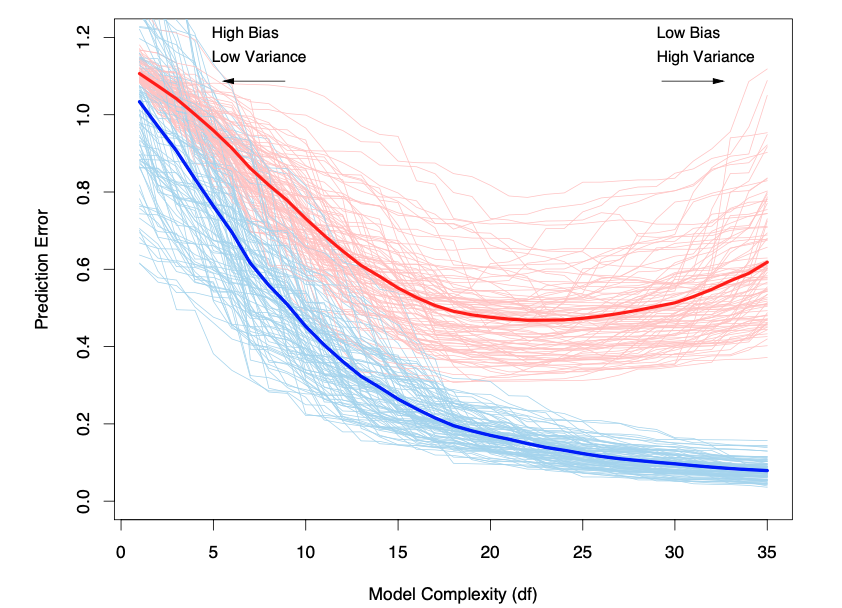
\includegraphics[width = 0.8\textwidth]{../assets/tibshirani7-1.png}
\end{figure}
\hfill \cite{hastie2009elements}

\textcolor{blue}{Blue} is in-sample error, \textcolor{red}{red} is out-of-sample error.

\end{frame}


%%%%%NOTE%%%%%
\note{
\scriptsize \singlespacing

\begin{itemize}
\item xxxx
\end{itemize}

}



%-------------------------------------------------------------------------------%
\begin{frame}{What is our goal in fitting a model?}

\begin{wideitemize}
\item We may want to use expected test error to \textbf{select among models}, or versions of models.\pause
\item And, once we have selected a version of a model, we may want to \textbf{assess} how a selected model performs. 
\end{wideitemize}

\end{frame}


%%%%%NOTE%%%%%
\note{
\scriptsize \singlespacing

\begin{itemize}
\item xxxx
\end{itemize}

}

%-------------------------------------------------------------------------------%
\begin{frame}{What is our goal in fitting a model?}

\begin{wideitemize}
\item We can't measure expected test error directly. 
\end{wideitemize}

\end{frame}


%%%%%NOTE%%%%%
\note{
\scriptsize \singlespacing

\begin{itemize}
\item xxxx
\end{itemize}

}

%-------------------------------------------------------------------------------%
\begin{frame}{What is our goal in fitting a model?}

\begin{wideitemize}
\item A procedure that allows us to estimate it:
\begin{itemize}
\item Split data into three parts
\begin{table}[]
\arrayrulecolor{white}  
\renewcommand{\arraystretch}{2.5}
\begin{tabular}{>{\centering\arraybackslash}p{5cm}|>{\centering\arraybackslash}p{2.5cm}|>{\centering\arraybackslash}p{2.5cm} }
\cellcolor{Contrast1l} \textcolor{white}{Training} & \cellcolor{Contrast4l} \textcolor{white}{Validation} & \cellcolor{Contrast6l} \textcolor{white}{Test} 
\end{tabular}
\end{table}
\pause
\item Fit models to the training set. \pause
\item Estimate prediction error of models in validation set. \pause
\item Select model with minimum error in validation set.\pause
\item Then get generalization error of just that model on test set. \pause
\end{itemize}
\item Why do we need to estimate the prediction error of the selected model \textit{again}? \pause Winner's curse. 
\end{wideitemize}

\end{frame}


%%%%%NOTE%%%%%
\note{
\scriptsize \singlespacing

\begin{itemize}
\item xxxx
\end{itemize}

}

%-------------------------------------------------------------------------------%
\begin{transitionframe}
\centering

\LARGE \textcolor{white}{Cross-validation.}

\end{transitionframe}
%-------------------------------------------------------------------------------%
\begin{frame}{Cross-validation.}

\begin{wideitemize}
\item We can potentially get more out of our data by cross-validating.
\end{wideitemize}

\begin{table}[]
\arrayrulecolor{white}  
\renewcommand{\arraystretch}{2.5}
\begin{tabular}{l >{\centering\arraybackslash}p{4cm}|>{\centering\arraybackslash}p{4cm} }
Version 1 & \cellcolor{Contrast1l} \textcolor{white}{Training} & \cellcolor{Contrast4l} \textcolor{white}{Validation} \\
\hline
Version 2 & \cellcolor{Contrast4l} \textcolor{white}{Validation} & \cellcolor{Contrast1l} \textcolor{white}{Training} \\
\end{tabular}
\end{table}
\pause

\[
\widehat{\textrm{Err}}_{CV} = \sum_{i = 1}^N L\left(y_i, \hat{f}^{-k(i)}(x_i) \right)
\]
$\hat{f}^{-k(i)}$ are the fits from the folds $k$ that do not contain $i$. 

\end{frame}


%%%%%NOTE%%%%%
\note{
\scriptsize \singlespacing

\begin{itemize}
\item xxxx
\end{itemize}

}

%-------------------------------------------------------------------------------%

\begin{frame}{K-fold cross validation.}

\begin{table}[]
\renewcommand{\arraystretch}{2.5}
\arrayrulecolor{white}  
\begin{tabular}{l >{\centering\arraybackslash}m{2cm} |>{\centering\arraybackslash}p{2cm}|>{\centering\arraybackslash}p{2cm}|>{\centering\arraybackslash}p{2cm}|>{\centering\arraybackslash}p{2cm} }
Version 1 & \cellcolor{Contrast1l} \textcolor{white}{Training} & \cellcolor{Contrast1l} \textcolor{white}{Training} & \cellcolor{Contrast1l} \textcolor{white}{Training} & \cellcolor{Contrast1l} \textcolor{white}{Training} & \cellcolor{Contrast4l} \textcolor{white}{Validation} \\
\hline
Version 2 & \cellcolor{Contrast1l} \textcolor{white}{Training}& \cellcolor{Contrast1l} \textcolor{white}{Training}& \cellcolor{Contrast1l} \textcolor{white}{Training} & \cellcolor{Contrast4l} \textcolor{white}{Validation} & \cellcolor{Contrast1l} \textcolor{white}{Training} \\
\hline
Version 3 &  \cellcolor{Contrast1l} \textcolor{white}{Training} & \cellcolor{Contrast1l} \textcolor{white}{Training}&\cellcolor{Contrast4l} \textcolor{white}{Validation}& \cellcolor{Contrast1l} \textcolor{white}{Training} & \cellcolor{Contrast1l} \textcolor{white}{Training} \\
\hline
Version 4 & \cellcolor{Contrast1l} \textcolor{white}{Training}& \cellcolor{Contrast4l} \textcolor{white}{Validation}& \cellcolor{Contrast1l} \textcolor{white}{Training}& \cellcolor{Contrast1l} \textcolor{white}{Training}  & \cellcolor{Contrast1l} \textcolor{white}{Training} \\
\hline
Version 5 & \cellcolor{Contrast4l} \textcolor{white}{Validation}& \cellcolor{Contrast1l} \textcolor{white}{Training}& \cellcolor{Contrast1l} \textcolor{white}{Training}& \cellcolor{Contrast1l} \textcolor{white}{Training}  & \cellcolor{Contrast1l} \textcolor{white}{Training} \\
\hline
\end{tabular}
\end{table}

\[
\widehat{\textrm{Err}}_{CV} = \sum_{i = 1}^N L\left(y_i, \hat{f}^{-k(i)}(x_i) \right)
\]
$\hat{f}^{-k(i)}$ are the fits from the folds $k$ that do not contain $i$. 


\end{frame}


%%%%%NOTE%%%%%
\note{
\scriptsize \singlespacing

\begin{itemize}
\item xxxx
\end{itemize}

}

%-------------------------------------------------------------------------------%
\begin{frame}{Cross-validion.}

\begin{wideitemize}
\item How do we pick $K$?\pause
\item $K = N$? \pause Low bias, possibly high variance (our prediction sets are very similar). \pause
\item $K = 5$? \pause Lower variance, possibly higher bias. \pause How much does the prediction change as we change the size of the data set?\pause
\begin{figure}
\centering
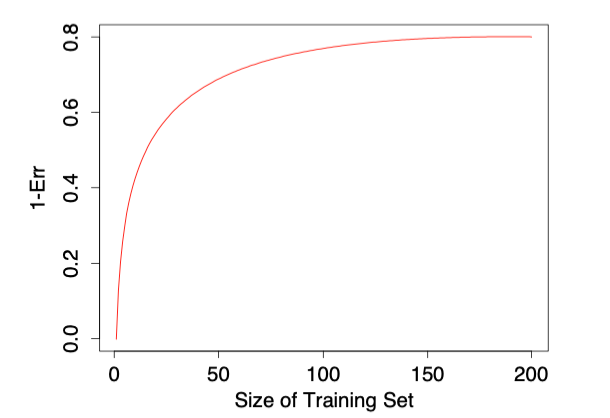
\includegraphics[width = 0.6\textwidth]{../assets/tibshirani7-8.png}
\end{figure}
\hfill \cite{hastie2009elements}
\end{wideitemize}

\end{frame}


%%%%%NOTE%%%%%
\note{
\scriptsize \singlespacing

\begin{itemize}
\item xxxx
\end{itemize}

}

%-------------------------------------------------------------------------------%
\begin{frame}{Cross-validion.}

\begin{wideitemize}
\item Rule of thumb is often 5 or 10.
\end{wideitemize}

\end{frame}


%%%%%NOTE%%%%%
\note{
\scriptsize \singlespacing

\begin{itemize}
\item xxxx
\end{itemize}

}

%-------------------------------------------------------------------------------%
\begin{transitionframe}
\centering

\LARGE \textcolor{white}{Bootstrapping.}

\end{transitionframe}
%-------------------------------------------------------------------------------%

\begin{frame}{Bootstrapping}


\begin{wideitemize}
\item Another approach, typically used to estimate the variability of an estimate over random samples, is bootstrapping.
\pause

\item If we knew the CDF of our population, we would be able to exactly determine the sampling variation of our estimate.
\pause

\item While we do not, we can  \textit{suppose} that the empirical CDF produced by the data that we observe is identical to the population CDF.
\pause

\item We can then just resample with replacement from our observed data, and see how much our estimates vary across resamples.
\end{wideitemize}

\end{frame}


%%%%%NOTE%%%%%


\note{
\scriptsize \singlespacing

\begin{itemize}
\item xxxx
\end{itemize}
}

%-------------------------------------------------------------------------------%
\begin{frame}{Bootstrapping for variability of the estimate due to random sampling}


The bootstrapping procedure is:

\begin{wideitemize}
\item For $b$ in $1\dots B$:
\begin{enumerate}

    \item Take a sample of size $N$  \textit{with replacement} from the observed data.\pause

    \item Apply the estimating procedure on the bootstrap sample.% to produce $\hat f^b$.
    \end{enumerate}
\pause

\item To get an estimate of the standard error of the estimate, calculate the standard deviation over these many bootstrap estimates.
\end{wideitemize}

\end{frame}


%%%%%NOTE%%%%%


\note{
\scriptsize \singlespacing

\begin{itemize}
\item xxxx
\end{itemize}
}

%-------------------------------------------------------------------------------%
\begin{frame}{Bootstrapping}

\begin{wideitemize}
\item How can we translate this method to estimate test error?
\end{wideitemize}

\end{frame}


%%%%%NOTE%%%%%
\note{
\scriptsize \singlespacing

\begin{itemize}
\item xxxx
\end{itemize}

}

%-------------------------------------------------------------------------------%
\begin{frame}{Bootstrapping for test error}


The bootstrapping procedure is:

\begin{wideitemize}
\item For $b$ in $1\dots B$:\pause
\begin{enumerate}

    \item Take a sample of size $N$  \textit{with replacement} from the observed data.\pause

    \item Apply the fitting procedure on the bootstrap sample to produce $\hat f^b$.
    \end{enumerate}
\pause
\item For each unit $i$, find the error from all of the bootstrap samples that do \textit{not} contain $i$.\pause
\[
\widehat{\textrm{Err}}_{Boot} = \frac{1}{N}\sum_{i = 1}^N \frac{1}{\lvert C^{-i} \rvert}\sum_{b \in C^{-i}} L(y_i, \hat f^b (x_i))
\]
$C^{-i}$ is the set of bootstrap samples that do not contain $i$, $\lvert C^{-i} \rvert$ is the size of this set.
\end{wideitemize}

\end{frame}


%%%%%NOTE%%%%%


\note{
\scriptsize \singlespacing

\begin{itemize}
\item xxxx
\end{itemize}
}

%-------------------------------------------------------------------------------%
\begin{frame}{Bootstrapping}

\begin{wideitemize}
\item How does the bootstrapping procedure perform?\pause
\item We still have the problem of too-small sample size\pause; on average, we only have $0.632 \times N$ unique observations in each boostrap sample. \pause
\item This means the bootstrap error \textit{over} estimates the test error. 
\item Solution: 
\[
\widehat{\textrm{Err}}_{0.632} = 0.368 \overline{\textrm{err}} + 0.632 \widehat{\textrm{Err}}_{Boot}  
\]
where $\overline{\textrm{err}}$ is the training error. \pause
\item This works...OK. \pause
\item Some alternatives in \cite{hastie2009elements}. 
\end{wideitemize}

\end{frame}


%%%%%NOTE%%%%%
\note{
\scriptsize \singlespacing

\begin{itemize}
\item xxxx
\end{itemize}

}

%-------------------------------------------------------------------------------%

\begin{transitionframe}
\centering

\LARGE \textcolor{white}{Bagging.}

\end{transitionframe}
%-------------------------------------------------------------------------------%
\begin{frame}{Bagging}

\begin{wideitemize}
\item We can combine estimates across samples to get smoother, or better estimators. \pause
\item \textcolor{Contrast6l}{\textbf{B}}ootstrap \textcolor{Contrast6l}{\textbf{agg}}regat\textcolor{Contrast6l}{\textbf{ing}}.
\end{wideitemize}

\end{frame}


%%%%%NOTE%%%%%
\note{
\scriptsize \singlespacing

\begin{itemize}
\item xxxx
\end{itemize}

}

%-------------------------------------------------------------------------------%
\begin{frame}{Bootstrap estimation for aggregated fit}

\begin{wideitemize}
\item For $b$ in $1\dots B$:\pause
\begin{enumerate}

    \item Take a sample of size $N$  \textit{with replacement} from the observed data. \pause

    \item Apply the fitting procedure on the bootstrap sample to produce $\hat f^b$.
    \end{enumerate}
\pause
\item The bagging estimate is 
\[
\hat f_{bag}(x) = \frac{1}{B}\sum_{i = 1}^N \hat f^b(x)
\]
\end{wideitemize}

\end{frame}


%%%%%NOTE%%%%%


\note{
\scriptsize \singlespacing

\begin{itemize}
\item xxxx
\end{itemize}
}

%-------------------------------------------------------------------------------%
\begin{frame}{Bagging}

\begin{wideitemize}
\item This is less interesting for something like a linear model, where $\hat f_{bag}(x) \to \hat f(x)$ as $B \to \infty$, since all of our observations are equally weighted in the sample, we'll reproduce the same thing\pause, or possibly a worse version of it. \pause
\item This is more interesting with something ``ragged'' like regression trees, where different trees can give us different branching behavior that we can smooth over. \pause 
\item If we're using a classifier, each model can get a ``vote'' for each $x$, and the class with the most votes wins. \pause
\item Or we can use averages of classifiers to produce probabilities, rather than just class predictions. 
\end{wideitemize}

\end{frame}


%%%%%NOTE%%%%%
\note{
\scriptsize \singlespacing

\begin{itemize}
\item xxxx
\end{itemize}

}

%-------------------------------------------------------------------------------%
\begin{frame}{Bagging}

\begin{wideitemize}
\item How many bootstrap replicates? \pause
\item 25? 50? \pause See how your results change with more replicates. 
\end{wideitemize}

\end{frame}


%%%%%NOTE%%%%%
\note{
\scriptsize \singlespacing

\begin{itemize}
\item xxxx
\end{itemize}

}

%-------------------------------------------------------------------------------%
\begin{transitionframe}
\centering

\LARGE \textcolor{white}{Honesty.}

\end{transitionframe}
%-------------------------------------------------------------------------------%
\begin{frame}{Honesty}

\begin{wideitemize}
\item Returning to (causal) inference\dots \pause we might like to use these methods to get valid inference, potentially on causal targets.
\end{wideitemize}

\end{frame}


%%%%%NOTE%%%%%
\note{
\scriptsize \singlespacing

\begin{itemize}
\item xxxx
\end{itemize}

}

%-------------------------------------------------------------------------------%
\begin{frame}{An honest tree algorithm}

\begin{enumerate}
\item Split the sample into two folds. \pause
\item Use the first fold to learn splits of the tree. \pause
\item Estimate response within leaves using the second fold. \pause
\end{enumerate}

\begin{wideitemize}
\item This can result in some leaves being empty. \pause Prune them? \pause
\item This procedure reduces bias relative to those proposed by \cite{breiman2001random}.
\end{wideitemize}

\end{frame}


%%%%%NOTE%%%%%
\note{
\scriptsize \singlespacing

\begin{itemize}
\item xxxx
\end{itemize}

}

%-------------------------------------------------------------------------------%
\begin{frame}[fragile]{An honest tree algorithm}

\begin{Schunk}
\begin{Sinput}
> library(grf)
> set.seed(60637)
> n <- 500
> p <- 10
> X <- matrix(rnorm(n * p), n, p)
> W <- rbinom(n, 1, 0.5)
> Y <- pmax(X[, 1], 0) * W + X[, 2] +
+   pmin(X[, 3], 0) + rnorm(n)
> c.forest <- causal_forest(X, Y, W)
\end{Sinput}
\end{Schunk}



\end{frame}


%%%%%NOTE%%%%%
\note{
\scriptsize \singlespacing

\begin{itemize}
\item xxxx
\end{itemize}

}

%-------------------------------------------------------------------------------%
\begin{frame}{An honest tree}

\begin{figure}
\centering
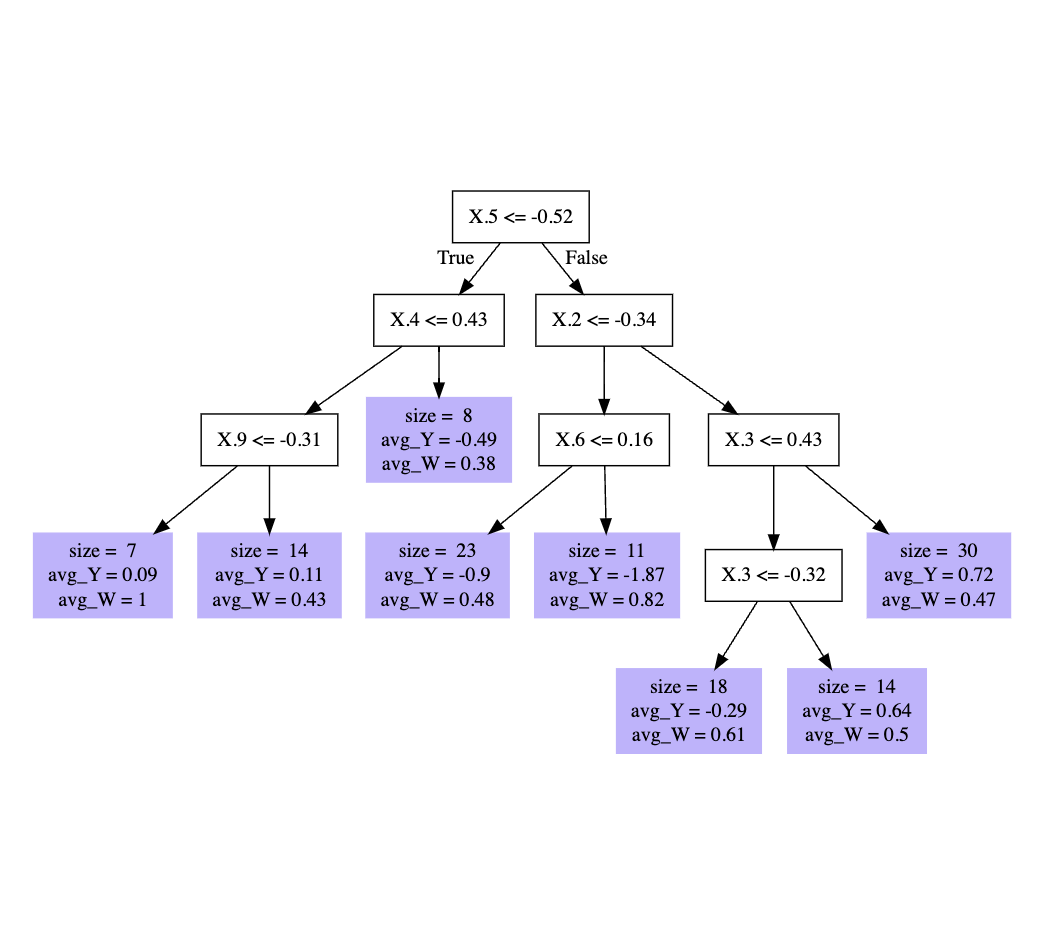
\includegraphics[width = 0.8\textwidth]{../assets/tree-plot.png}
\end{figure}
\hfill
\end{frame}


%%%%%NOTE%%%%%
\note{
\scriptsize \singlespacing

\begin{itemize}
\item xxxx
\end{itemize}

}

%-------------------------------------------------------------------------------%


\backupbegin
%-------------------------------------------------------------------------------%

\begin{frame}[allowframebreaks]{References}
    \bibliographystyle{apalike}
    \bibliography{../assets/PLSC40601}
\end{frame}
%-------------------------------------------------------------------------------%
\backupend
\end{document}
%
%-------------------------------------------------------------------------------%
%%% [[TEMPLATE]] %%%
\begin{transitionframe}
\centering

\LARGE \textcolor{white}{Statement.}

\end{transitionframe}
%-------------------------------------------------------------------------------%

%%% [[TEMPLATE]] %%%
\begin{frame}{Frametitle}

\begin{wideitemize}
\item xxx
\end{wideitemize}

\end{frame}


%%%%%NOTE%%%%%
\note{
\scriptsize \singlespacing

\begin{itemize}
\item xxxx
\end{itemize}

}

%-------------------------------------------------------------------------------%
